\documentclass[a4paper,11pt]{report}

%%%%%%%%%%%%
% packages %
%%%%%%%%%%%%
\usepackage{caption}
\usepackage{color}
\usepackage[english]{babel}
\usepackage[utf8x]{inputenc}
\usepackage{lmodern}
\usepackage[T1]{fontenc}

\usepackage{listings}
\usepackage{microtype}
\usepackage{avant}

\usepackage{graphicx}
\usepackage{fancyhdr}
\usepackage{pgfgantt}

%% Maths symbols
\usepackage{amsmath}
\usepackage{amssymb}

% float figures forcing
\usepackage{placeins}
% GNUPLOT
%\usepackage{gnuplot-lua-tikz}

\usepackage{sectsty}

%%%%%%%%%%%%%%%%%%%
% custom commands %
%%%%%%%%%%%%%%%%%%%
\newcommand{\HRule}{\rule{\linewidth}{0.5mm}}
%\usepackage[left=3cm,right=3cm,top=2cm,bottom=2cm]{geometry}
\usepackage{geometry}


%%%%%%%%%%%%%%
% new colors %
%%%%%%%%%%%%%%
% solarized colors
\definecolor{base03}{HTML}{002B36}
\definecolor{base02}{HTML}{073642}
\definecolor{base01}{HTML}{586E75}
\definecolor{base00}{HTML}{657B83}
\definecolor{base0}{HTML}{839496}
\definecolor{base1}{HTML}{93A1A1}
\definecolor{base2}{HTML}{EEE8D5}
\definecolor{base3}{HTML}{FDF6E3}
\definecolor{yellow}{HTML}{B58900}
\definecolor{orange}{HTML}{CB4B16}
\definecolor{red}{HTML}{DC322F}
\definecolor{magenta}{HTML}{D33682}
\definecolor{violet}{HTML}{6C71C4}
\definecolor{blue}{HTML}{268BD2}
\definecolor{cyan}{HTML}{2AA198}
\definecolor{green}{HTML}{859900}

\definecolor{defaultFontColor}{HTML}{073642} % base 02

%%%%%%%%%
% fonts %
%%%%%%%%%
% inconsolata %
\usepackage{inconsolata}
%\renewcommand*\familydefault{\ttdefault} %% Only if the base font of the document is to be typewriter style
%\usepackage[T1]{fontenc}
\renewcommand*\familydefault{\rmdefault}\color{defaultFontColor} %% Only if the base font of the document is to be typewriter style

\chapterfont{\color{red}}
\sectionfont{\color{orange}}
\subsectionfont{\color{blue}}
\paragraphfont{\color{base01}}
\paragraphfont{\color{base2}}
\subparagraphfont{\color{base2}}

% title specific %
% title rule
\newcommand{\titleRule}{\color{base2}\HRule\color{defaultFontColor}}

%%%%%%%%%%%%%%%%%%%%
% listing settings %
%%%%%%%%%%%%%%%%%%%%
\lstset{
    basicstyle=\ttfamily,
    language=c,
    frame=lines,
    sensitive=true
    tabsize=2,
    breaklines=true,
    showstringspaces=false,
    showspaces=false,
    numbers=left,
    backgroundcolor=\color{base3},
    keywordstyle=\color{cyan},
    commentstyle=\color{base1},
    stringstyle=\color{blue},
    numberstyle=\color{violet},
    rulecolor=\color{base00},
    morekeywords={nm}
}

%%%%%%%%%%%%%%%%%%%%
% caption settings %
%%%%%%%%%%%%%%%%%%%%
\DeclareCaptionFont{captionText}{\color{base1}}
\DeclareCaptionFormat{listing}{\colorbox{base03}{\parbox{\textwidth}{\hspace{15pt}#1#2#3}}}
\captionsetup[lstlisting]{format=listing,labelfont=captionText,textfont=captionText, singlelinecheck=true, margin=0pt, font={sf,footnotesize}}
\DeclareCaptionFormat{figure}{\colorbox{base03}{\parbox{\textwidth}{\hspace{15pt}#1#2#3}}}
\captionsetup[figure]{format=figure,labelfont=captionText,textfont=captionText, singlelinecheck=false, margin=0pt, font={sf,footnotesize}}

%%%%%%%%%%%%%%%%%%%%%%
% pagestyle settings %
%%%%%%%%%%%%%%%%%%%%%%
\pagestyle{fancy}
\renewcommand{\headrulewidth}{0.4pt}
\fancyhead{}
\fancyhead[LE]{\textit{\nouppercase{\leftmark}}}
\fancyhead[RO]{\textit{\nouppercase{\rightmark}}}
\fancyfoot{}
\fancyfoot[C]{\thepage}

\usepackage{hyperref}
% Hyperref setup
\hypersetup{colorlinks=true}
\hypersetup{urlcolor=blue}
\hypersetup{citecolor=dkgreen}

%%%%%%%%%%%%%%%%%%%%%%%%
% custom environnments %
%%%%%%%%%%%%%%%%%%%%%%%%
\newenvironment{sectionIntro}{\textsf}{\newline}
\newenvironment{figureGraphics}[2]
{\begin{figure}[h!] \caption{#1} \label{#2} \centering}%
{\color{base03}\hrule\end{figure}\FloatBarrier}

%%%%%%%%%%
% Biblio %
%%%%%%%%%%
\bibliographystyle{alpha}

%#############################################################################%
% End of preamble                                                             %
%#############################################################################%

\begin{document}
\begin{titlepage}


% Upper part of the page

\begin{minipage}{\textwidth}

\includegraphics[width=0.30\textwidth]{./src/img/logoups.jpg}
\hfill 
\includegraphics[width=0.20\textwidth]{./src/img/logointel.jpg} \hfill

\includegraphics[width=0.25\textwidth]{./src/img/logocelad.jpg}
\end{minipage}

\begin{center}
% Irit logo
%\includegraphics[width=0.40\textwidth]{./src/img/logoIRIT}\\[0.3cm]
%\textsc{\Large Team SEPIA}\\[1.5cm]

\vfill

\textsc{\LARGE Internship report}\\[0.5cm]

% Title
\titleRule \\[0.4cm]
{ \huge \bfseries Android middleware \& sofware development, integration \& tests}\\[0.4cm]

\titleRule \\[1.5cm]

\vfill

% Author and supervisor
\begin{minipage}{0.4\textwidth}
\begin{flushleft} \large
\emph{Intern:}\\
Mattijs Korpershoek\\
\href{mailto:mattijs.korpershoek@gmail.com}{mattijs.korpershoek@gmail.com}\\
Université Paul Sabatier\\
\end{flushleft}
\end{minipage}
\begin{minipage}{0.4\textwidth}
\begin{flushright} \large
\emph{At} \\
Intel Toulouse \\
\emph{on behalf of}\\
CELAD\\
\end{flushright}
\end{minipage}

\vfill

\emph{Master CAMSI}\\
Year 2013 - 2014

\end{center}

\end{titlepage}

\hypersetup{linkcolor=defaultFontColor}
\tableofcontents
\hypersetup{linkcolor=blue}
\newpage

\chapter*{Forewords}

Thanks to


Thanks to


Thanks to *** for ***

\chapter{Introduction}

\lstinputlisting[caption=A simple hello world]{./src/hw.c}

\chapter{Context}

Introduction of this part.

\section{CELAD}

\section{Intel}
\subsection{Opensourcing}
Contribution leader to kernel 3.14, ...

\subsection{Android}

\subsection{Audiocomms feature team}
 % WHERE I DID the work, and on what
\chapter{Organisation}\label{chap:organisation}

\section{Planning}
\subsection{Discovering the code}
At the first work week, I dug into the Parameter-framework's code. I had no
documentation at all, just the code on GitHub. The absence of help was done on
purpose: the team needed an external point of view on the source code. I had
to understand the powerful concepts of the Parameter-framework just by reading
the code. Since I struggled a bit with the concepts, I decided to write some
newcomer tutorials which content are described at section \ref{sec:tutorials}.

\subsection{Joining forces with the scrum team}
After three weeks, I requested to join a scrum team so that I could experience
Intel's way of working with scrum! I did the rest of my internship as an agile developer,
working the same way as the other team members.

\subsection{Gantt}
TODO REWORK
\begin{ganttchart}[
        x unit=0.5cm,
        y unit title=.6cm,
        y unit chart=.6cm,
        hgrid=true,
        vgrid={*1{red,  dotted}},
        canvas/.style={fill=base2},
        bar/.style={fill=orange},
        title/.style={fill=base2},
        group/.style={fill=blue, shape=ganttgroup},
        bar height = 0.4,
    ]{1}{24}
    \gantttitlelist{1, ..., 24}{1} \\
    \ganttgroup{GitHub}{1}{4} \\
    \ganttbar{Installation}{1}{2} \\
    \ganttbar{Découverte PFW}{1}{4} \\
    \ganttgroup{Android}{4}{9} \\
    \ganttbar{XML validation}{4}{8} \\
    \ganttbar{Code checker}{6}{7} \\
    \ganttbar{HW detection}{8}{9} \\
    \ganttbar{Fixed point improvements}{9}{13} \\
    \ganttbar{Build system issues}{11}{13} \\
    \ganttbar{Alsa plugin refactor}{13}{15} \\
    \ganttbar{PFW IP plan}{13}{14} \\
    \ganttbar{File system plugin}{14}{15} \\
    \ganttbar{PFW Core}{16}{18} \\
    \ganttbar{Xmm plugin}{18}{19} \\
    \ganttbar{Vacances}{21}{21} \\
    \ganttbar{Internship report}{22}{24} \\
\end{ganttchart}

\section{Agile methodology}

In the team I was working, we were organized around Agile software
development. This way of working promotes incremental results and adaptive planning.
There are several implementations of Agile methods. In our team we were using Scrum.

In order to understand how I worked during my internship, some key concepts of Scrum must be described.

\subsection{Core concepts}

\subsubsection{Story}\label{sec:story}
A story is a \emph{business-oriented}, short description of a client's
need. Most of the times, it is divided into several tasks so that the developers
can take small steps to complete the story. A story is usually printed or
written on sticky note. Those notes are grouped on a story board.

\begin{figureGraphics}{A story board}{fig:storyboard}
    TODO picture of a story board
\end{figureGraphics}


\subsubsection{Sprints}\label{sec:sprint}
Sprints are short development cycles, usually from one to four weeks. We were
delivering results every three weeks. During each sprint, a team creates a
shippable product, no matter how basic that product is. A sprint is composed of
a set of stories which should be completed at it's end.

The interesting part of working in sprints is the idea of "making a fresh start" every three weeks. This
was quite motivating to me!


\subsection{Team}
Our team is composed of six members(me included); all software engineers with various
skills. Some are more software design oriented while others are more hardware
specialists.

In a Scrum, some members have a particular role:
\begin{description}
    \item[The Product owner]
        defines what the team is doing during a Sprint (see \ref{sec:sprint}).
        He determines the priority of each story (see \ref{sec:story}) the team is working on. His input usually comes from
        clients. He is the business-oriented person in the team. His decisions have an impact on the results a Scrum team delivers.
    \item[The Scrum master]
        ensures that every team member is correctly focused on his story. He is keeping track of the progress of each member and
        should alert the Product owner when some planning issues occur (bad time estimation, very urgent incoming task, ...).
\end{description}

Note that in our team, the Product owner and the Scrum master were also contributing to the team as software engineers.

\subsection{Events}
In Scrum, there are several events occurring during a sprint.
These are essential to the scrum methodology.

\subsubsection{Daily scrum}
Every day, at 11:30 we were holding the daily scrum meeting, also called "stand-up".
During that time, each member of the team answers quickly the three following questions:

\begin{description}
    \item[What have I done since yesterday ?]
    \item[What am I planning for today ?]
    \item[Any issues encountered ?]
\end{description}

This meeting is very useful, it helps tackle early problems and can assist the scrum master to detect delays in delivering.
Note that this should not take longer than 15 minutes.


\subsubsection{Planning poker}
During planning poker sessions, we have to estimate how much time each story takes. In order to do a correct estimate,
the product owner is explaining what the exact requirements are. After that, each member of the team should guess
how much "story points" (which can sometimes be approximated to a day of work) the story should take to be done.
This is done in the form of a vote, with poker session cards.

\begin{figureGraphics}{Planning poker cards}{fig:poker}
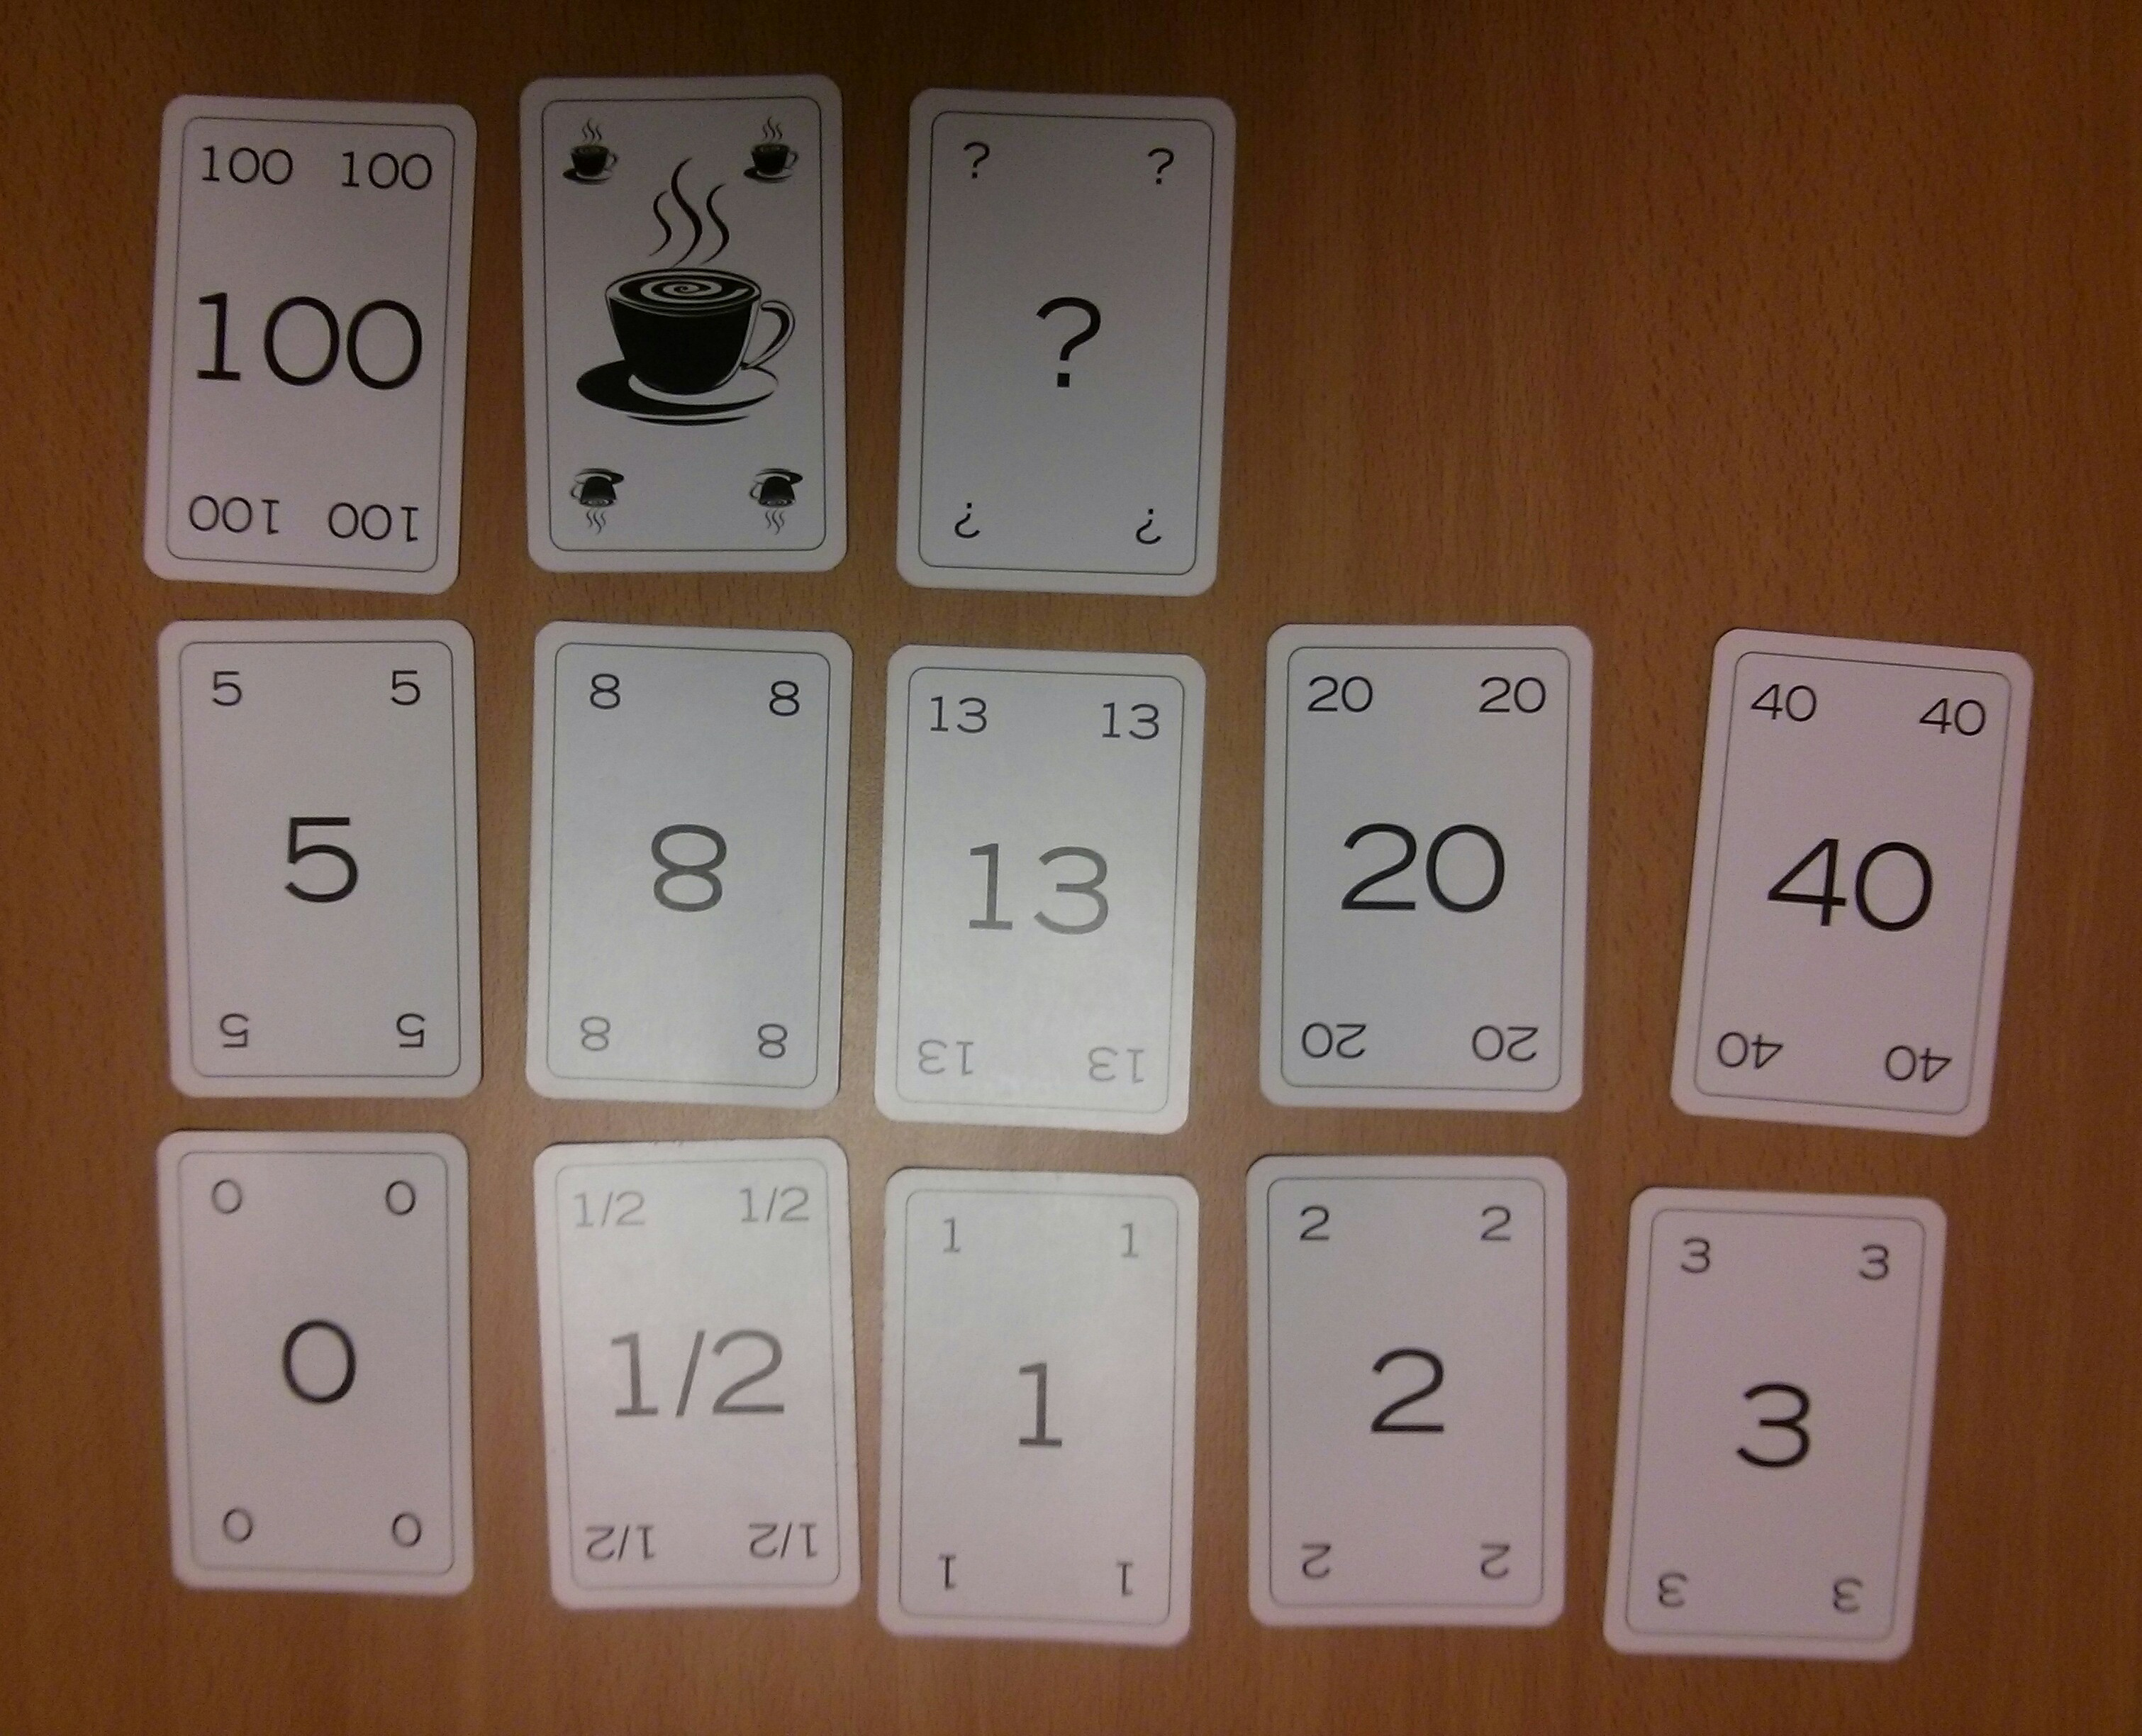
\includegraphics[width=\textwidth]{./src/img/poker.jpg}
\end{figureGraphics}

After arriving at a team consensus, the story is considered \emph{planned}. This
is very useful so that the Product owner can group multiple stories which have
to be done in a sprint.


\subsubsection{Demos}
At the end of each sprint, the team has to demonstrate their achievements. This
is a very important meeting with people external to the team. Only the work
which was \emph{done} during the last sprint is showed off during that presentation.

This presentation is important to show the contributions that the team has made.
I participated in every Demo since I was fully member of the scrum team.

\subsubsection{Retrospectives}
After the Demo, the team has a look back at how the last sprint happened. This short meeting is made
to find out what the team did wrong last sprint, but also to highlight what the team did right!
It is frequent to see little psychological games during the retrospective, which makes all members more
eager to participate.

\section{Workflow}
In this section, we will see how I was working during my internship.

\subsection{Setup}
Since compiling the Android source tree requires a lot of computing power,
most of developers of our team are working remotely, via ssh.
The server we are connecting to is far more powerful than the desktops we use.
With it 32 cores and it's 2 TeraBytes of SSD, compilation time was far less time-consuming
than compiling locally!

I also worked via that server, everything via command-line interface, as showed below.
\begin{figureGraphics}{Development setup with vim and tmux}{fig:setup}
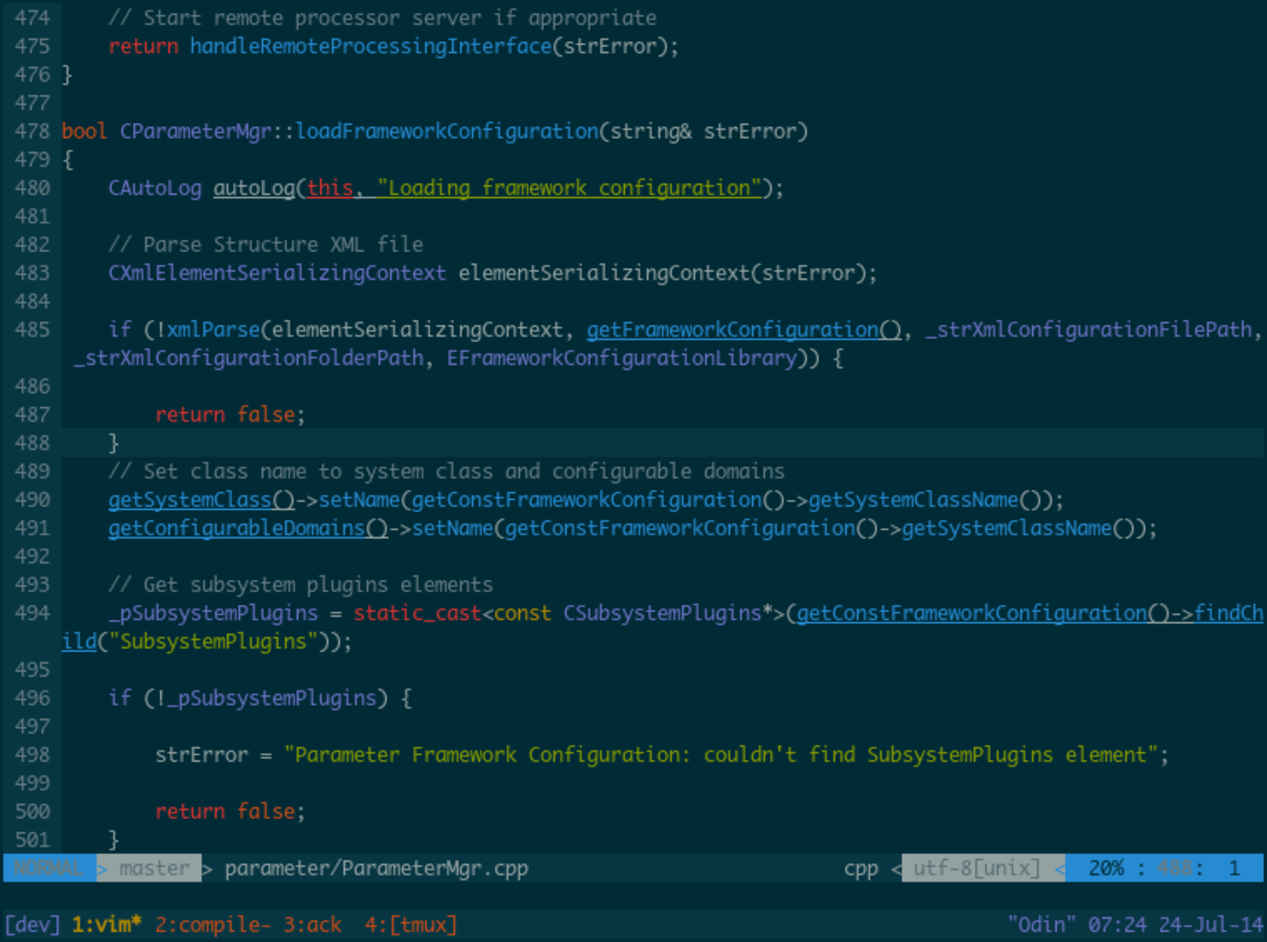
\includegraphics[width=\textwidth]{./src/img/setup.pdf}
\end{figureGraphics}

\subsection{Development}
During the
\subsection{Verification}
\subsection{Review}
\subsection{Pre-integration}
 % HOW I PLANNED the work
\chapter{Contributions}\label{chap:contributions}

All the work I have done during this internship is related to the \gls{pfw},
which was briefly presented in section \ref{sec:parameter-framework}.
I had two major directions during my internship:
\begin{itemize}
    \item Delivering new features for Intel and its customers.
        I have submitted more than \emph{80 patches} to the Intel codebase, which are now used by its customers.
    \item Open-sourcing the \gls{pfw} to give it some weight in the middleware community.
        For doing that, I had to change some code within the \gls{pfw}.
        Today, I am in the top five contributors on GitHub as shown on figure \ref{fig:githubContrib} below (My nickname is \emph{Makohoek}).
        \begin{figureGraphics}{Top contributors on the Parameter-framework core}{fig:githubContrib}
            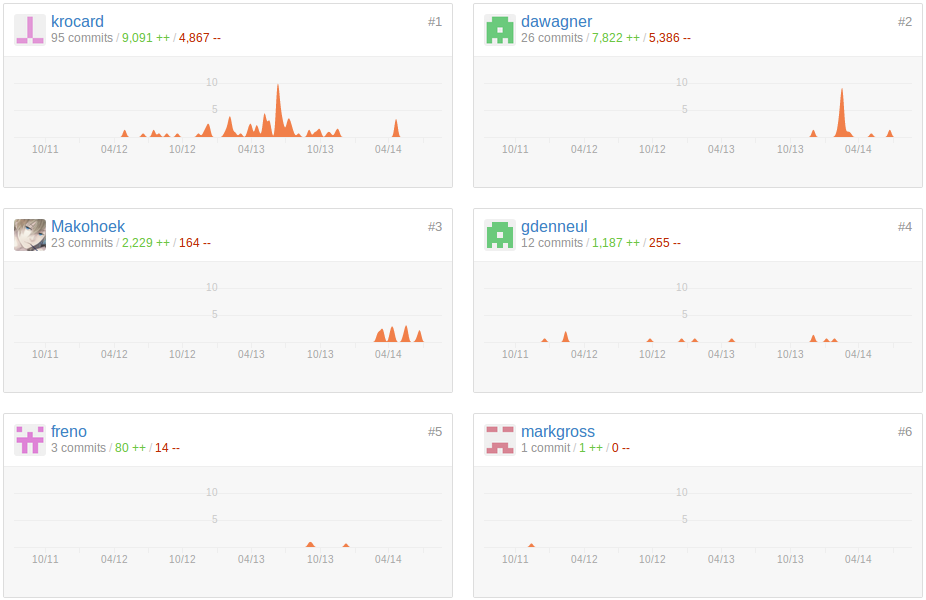
\includegraphics[width=\textwidth]{./src/img/statsGitHub.png}
        \end{figureGraphics}
\end{itemize}

% {{{1 CLIENT FEATURES
\section{New features for Intel and its customers}

In this section, I will detail the different problems I solved for Intel and its customers.
The code I delivered is currently used by several customers and respects high software quality standards
as described in section \ref{sec:quality}

% {{{2 Xml validation at build time
\subsection{XML validation at build time}

For our Intel Audio \gls{hal}, we have a lot of structure files. More than one hundred, which represents
more than 40 000 lines of \gls{xml} files.
The writing of those structure files is done by human beings. Given the fact
that humans can make mistakes, there is \emph{no guarantee} that those structure files are semantically correct.
Furthermore, the \gls{pfw} expects that the files which are given do not contain any mistake.

An example can be that someone forgot to specify the \emph{size} attribute of a parameter.
In that case, the default size is $0$. Let's imagine we are computing a result as showed in figure \ref{fig:runtimeerror}.

\begin{figureGraphics}{Error example due to a bad parameter size}{fig:runtimeerror}
    $result = \dfrac{a*k}{size}$
    \vspace{0.3cm}
\end{figureGraphics}

In that case we have a run-time error due to a \emph{division by zero}. This is only one possible consequence of bad structure files.
This kind of problem should be detected at build-time, not at run-time. Having those problems at
run-time is far too time-consuming and thus far too expensive.

In the next sections we will see how to detect those problems at build time.

\subsubsection{A language for validating XML files}

To validate \gls{xml} files, we use \gls{xsd} files.
Those are describing what is allowed/prohibited within an \gls{xml} element. For example, the \emph{size} attribute is
\emph{mandatory} for an Integer parameter.
Listing \ref{lst:xsd} shows a snippet illustrating that example \gls{xsd} file:

\begin{code}[language=XML, caption=XSD rules for an Integer parameter, label=lst:xsd]
<xs:attributeGroup name="IntegerParameterAttributes">
    <xs:attribute name="Size" type="SizeType" use="required"/>
    <xs:attribute name="Min" type="xs:integer" use="optional"/>
    <xs:attribute name="Max" type="xs:integer" use="optional"/>
    <xs:attribute name="Signed" type="xs:boolean" use="optional" default="false"/>
</xs:attributeGroup>
\end{code}

With that knowledge in mind, I decided to write a \gls{python} tool to detect the possible errors in the existing structure files.

\subsubsection{A tool to validate XML}
To validate \gls{xml} with \gls{xsd} files, several tools already exist. The most widely used on linux is the \lstinline{xmllint} utility.
This works very well but is limited to one file per usage. The script I wrote in \gls{python} was able to have two directories as input and check
recursively every file.
This tool highlighted that there were more than \emph{500 errors} within the hundred files.

This \gls{python} script worked great, but it had an issue. It did \emph{not use standard} \gls{python} libraries.
Since this had to run on many different machines(more than a thousand), it was out of question to install those third-party libraries everywhere.
We needed a more robust solution which was integrated into the build system without using external libraries.

\subsubsection{Build process}
To understand how the robust solution is implemented, we need to have a look at the build process around the \gls{pfw}.

During the build process, we are translating settings files from a special format (which was shown in \ref{lst:pfwsettings}) into \gls{xml}.
That special format, which is called \emph{.pfw language}, is used for rule based
description. Those are translated into \gls{xml} files during the build via a
specific make target.  In order to generate those \gls{xml} files, we also need
the information of the structure files, which are written by the integration
engineers as described in previous subsection.

To generate those files, we rely on a toolset we call \emph{HostDomainGenerator}.
The figure \ref{fig:build-process} shows how it works:

\begin{figureGraphics}{Xml generation build process}{fig:build-process}
    \includegraphics[height=0.4\textheight]{./src/img/build-generation.pdf}
\end{figureGraphics}

\begin{itemize}
    \item The \emph{.pfw} files are parsed via a set of scripts and translated into \gls{pfw} commands.
    \item Those commands are sent to a special \gls{pfw} instance which was started for this purpose only.
    \item After that, the \gls{pfw} exports the rules which have previously been created and dumps it into a settings \gls{xml} file.
    \item Those \emph{settings} and \emph{structure} files are then stored on the smartphone or the tablet on the file-system.
\end{itemize}

In this build process, we have to display errors when detecting \gls{xml} files which are not compliant with the rules from the
\gls{xsd} files.

\subsubsection{Xml checker}

Since we wanted a more robust solution, it was finally done within the \gls{pfw} itself.
In fact, the parameter-framework had already some code to check \gls{xml} validity. It was not
finished and I had to complete it.

When that was done, I had to integrate the feature within the \lstinline{HostDomainGenerator} tool.
Figure \ref{fig:build-process-reworked} shows the final implementation.

\begin{figureGraphics}{Xml generation build process with validity check}{fig:build-process-reworked}
    \includegraphics[height=0.5\textheight]{./src/img/build-generation-after.pdf}
\end{figureGraphics}

With the difference to the solution showed in figure \ref{fig:build-process}, here we:
\begin{itemize}
    \item Give \gls{xsd} files towards the \lstinline{hostDomainGenerator} tool.
    \item Those are forwarded to the \gls{pfw}, which validates the \emph{structure} files before receiving the special commands.
    \item If the validation fails, it aborts the build.
    \item Otherwise, it dumps the \emph{settings} file as usual.
\end{itemize}

\subsubsection{Outcome}
In the end, this solution is widely used at Intel now. All errors described by the \gls{xsd} rules have been removed.
In a matter of two weeks, the integration team was able to clean up more than 500 errors from the \gls{xml} structure files.
Moreover, it is impossible nowadays to let new validation errors go trough, since the system would not build.


% {{{2 Multivariance
\subsection{Multi-variant initial support}
\subsubsection{Context}
Intel has a various number of platforms for smarphones and tablets, which have different hardware specifications.
Each platform also haves minor hardware variances.
For example, there is a platform with two hardware variants: the audio architecture is not the same.
The architecture can for instance differ in a codec. Each of those different combinations is called a \emph{variant}.

A customer requirement was to be able to have one single package for the Intel Audio \gls{hal} which works on every variant.
With this concern in mind, we had to rework the \gls{hal} a bit.
In fact, as seen in section \ref{sec:parameter-framework}, the \gls{pfw} needs \gls{xml} files which are hardware dependent.

Within the our build system, we are aware of which \gls{xml} files should be loaded, since that depends on the variant we are building.
So, for each variant, we build a different package which includes the correct \gls{xml} files.
This had to be reworked into a single package.

\subsubsection{Implementation}
For an initial step, we decided to include every \gls{xml} file for all the possible variants.
The problem is that at run-time, the Stream manager (which is in the \gls{hal}) has \emph{no idea} about which configuration file
it should load for his \gls{pfw} instance.

The Stream manager needs to be smarter. In our case, as each variant has a different sound card name, we decided to
rely on this information to decide which configuration of the \gls{pfw} would be loaded.
In order to detect what the current sound card is, we can read from \lstinline{/proc/asound} entries.
The current implementation relies on the content of \lstinline{/proc/asound/cards}.
We have a map in the Stream manager which has as key the \emph{sound card name} and as value the \gls{xml} file which should be loaded.
This is viable since there are less than five hardware variances at most for each platform.

This is just a proof of concept to show to customers that we are able to support multiple hardware variants with one single package.


% {{{2 Fixed point param
\subsection{Fixed point parameter improvements}
% What are fixed points
% Problem
Fixed point numbers are useful for representing real numbers. Their
usage is appropriate when the processor does not have a floating point unit
or when there is a performance gain by using them. Usually, fixed points are
represented by $Qn.m$ format, where $n$ is the \emph{Integral part} and $m$ the
\emph{Fractional part}.

The implementation of fixed point numbers in the \gls{pfw} has some
corner cases which were not correctly handled. Round issues appeared when we
were writing to a configuration file or displaying user input. To
support the expected behavior for those cases, I changed the implementation, and
wrote tests for it.

\subsubsection{The problem}
The \gls{pfw} can export parameters to a file. It has several parameter types.
Fixed point number have their own type, called \emph{FixedPointParameters}. Of course, they can be exported as well.
\begin{itemize}
    \item When exporting a \lstinline{FixedPointParameter} to a file, the \gls{pfw} converts the value from
        its internal representation towards a floating point number, because that is
        easier to read.
    \item By converting that number, it also computes the amount of digits needed to display (or write) that number.
        This results in \emph{rounding issues}, due to limitation of the \lstinline{setPrecision()} \gls{cpp} method.
        In fact, \lstinline{setPrecision()} is \emph{rounding up} instead of \emph{truncating} the last digit of a floating point number.
        For instance:
        \begin{itemize}
            \item \lstinline[language=C++]{cout << setPrecision(3) << 3.14159265} returns $3.14$.
            \item \lstinline[language=C++]{cout << setPrecision(5) << 3.14159265} returns $3.1416$ instead of $3.1415$.
        \end{itemize}
        It is not possible to change the \emph{rounding} behavior to \emph{truncating} behavior because
        \lstinline{setPrecision()} relies on the \lstinline{fesetround()} methods which is only available in the \gls{cpp} 11 norm.
\end{itemize}
In the next section we will study an example showing the issue.

\subsubsection{An example of the issue}

Let's take the case of a $Q2.3$ number: the \emph{Integral part} is $2$ and the
\emph{Fractional part} is $3$.
Since we have a fractional part of $3$ bits, the minimal step between two numbers coded in $Q2.3$ is
$2^{-3}$. This minimal step is called the \emph{Quantum}.

Some special values can be represented for a $Q2.3$ number. Figure \ref{fig:fixedPointValues} below shows those values. Note that
this figure is not represented in real scale.
\begin{figureGraphics}{Fixed point special values}{fig:fixedPointValues}
    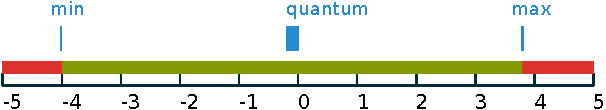
\includegraphics[width=\textwidth]{./src/img/fixedPoint.pdf}
\end{figureGraphics}

\begin{itemize}
    \item The Quantum is $2^{-3} = 0.125$
    \item The UpperBound is $2^2 - Quantum = 3.875$.
        This implies that it should be \emph{impossible} to set a larger value than $3.875$.
    \item The LowerBound is $-2^2 = -4$.
        This implies that it should be \emph{impossible} to set a smaller value than $-4$.
\end{itemize}

With those values, we can illustrate the issue.
Listing \ref {lst:fixedPointProblem} below exposes the problem.

\begin{code}[language=bash, caption=$Q.2.3$ rounding issue example, label=lst:fixedPointProblem]
# Let's set the maximum allowed value
$ pfw setParameter /Example/fixedPoint/q2.3 3.875
# Done
$ pfw getParameter /Example/fixedPoint/q2.3
# 3.9
# ^ this is not expected,
# ^ since 3.875 is an encodable number for Q2.3!

# Ok, let's try to set the number the pfw gave us:
$ pfw setParameter /Example/fixedPoint/q2.3 3.9
# Value 3.9 standing out of admitted real range
# [-4, 3.875] for FixedPointParameter /Test/test/q2.3
# ^ We are NOT able to set something the pfw gave us!
\end{code}


\subsubsection{A test suite to describe valid behavior}

In order to verify that the new implementation would be correct, I wrote a test suite
in \gls{python}. That test suite performs several checks on each fixed point. Let's
take the previous example to illustrate the mechanics of the test suite.

The test suite uses two types of data to handle its test:
\begin{description}
    \item[Out-of-bound values] which should be \emph{refused} by the \gls{pfw}.
    \item[Inner bounds values] which should be \emph{accepted} by the \gls{pfw}.
\end{description}

Figure \ref{fig:fixedPointTest} below illustrates the flow of the two types of tested data.

\begin{figureGraphics}{fixed point test suite}{fig:fixedPointTest}
    \includegraphics[height=0.6\textheight]{./src/img/fixedPointProcess.pdf}
\end{figureGraphics}

The checks are done as following:
\begin{description}
    \item[Bound check] The \gls{pfw} should throw an error if we
        attempt to set an out-of-bound value.
    \item[Sanity check] If we manage to set the value, The \gls{pfw} should not modify too much
        the value. It can change by half a quantum at maximum.
    \item[Consistency check] The \gls{pfw} should accept the value it sent previously.
    \item[Bijectivity check] The \gls{pfw} should return the same value we provided it at the Consistency check.
\end{description}

\subsubsection{The solution}
The fix I proposed was to replace the calculation of the amount of displayed digits.
Since it had problems with rounding, why not show all digits at the end of the number?

The \emph{fractional part} of a $Qn.m$ number is always a multiple of its quantum. This is related to
the internal representation of fixed point numbers. Since a quantum is always a number in the form of $2^{-m}$, we can
assume that the quantum's last digit will aways be a $5$, for $m > 0$.

Figure \ref{fig:quantums} below shows some possible quantum values, where $m$ is the \emph{fractional part} of a $Qn.m$:

\begin{figureGraphics}{Quantum values}{fig:quantums}
    $
    \begin{array}{c|c}
        m & Quantum = 2^{-m} \\
        \hline
        1 & 0.500000 \\
        \hline
        2 & 0.250000 \\
        \hline
        3 & 0.125000 \\
        \hline
        4 & 0.062500 \\
        \hline
        5 & 0.031250 \\
        \hline
        6 & 0.015625
    \end{array}
    \vspace{0.3cm}
    $
\end{figureGraphics}

So we can assume that the quantum last digit is always $5$.
It happens that that last digit is always the $m^{th}$ digit after the comma.
So we just need to call \lstinline{setPrecision(m)} with $m$ as \emph{fractional part} of a $Qn.m$.
Listing \ref{lst:resultFixedPoint} shows the correct interaction with the \gls{pfw} command-line interface.

\begin{code}[language=bash, caption=$Q.2.3$ correct set and get, label=lst:resultFixedPoint]
# Let's set the maximum allowed value
$ pfw setParameter /Example/fixedPoint/q2.3 3.875
# Done
$ pfw getParameter /Example/fixedPoint/q2.3
# 3.875
# ^ Ok, correct behavior

# Let's try to set a different value:
$ pfw setParameter /Example/fixedPoint/q2.3 3.8
# Done
$ pfw getParameter /Example/fixedPoint/q2.3
# 3.750
# ^ Ok, this is acceptable since 3.8 is not encodable.

# Let's try to set a erronous value:
$ pfw setParameter /Example/fixedPoint/q2.3 3.9
# Value 3.9 standing out of admitted real range
# [-4, 3.875] for FixedPointParameter /Test/test/q2.3
# ^ This also correct
\end{code}

\subsubsection{Outcome}

The current implementation is used at daily basis by multiple tools.
More than \emph{80 structure files} which are also for Intel's customers are compatible with this solution.
This was a complex issue that caused the team a few weeks of effort and I am proud that my answer has been the
correct one to this problem.


% {{{2 Multi modem
\subsection{Multiple modem support}
\subsubsection{Context}
With the \emph{bring your own device} trends, more and more smartphones support dual simcards. This case
is useful to use the same device for corporate and private purposes.
Besided, in some developing countries phone carriers do not cover the whole country. The habitants of those
countries need several phone carriers to use their smartphone smoothly.
For those purposes, the platform must support two modems.
Within the Intel Audio \gls{hal}, we are handling some voice processing algorithms from the signal coming from the modem.
Naturally, we have a \gls{pfw} plugin to abstract the modem. This plugin did not support multiple modems.

I had to add \emph{modem instance awareness} to the plugin so that Intel could ship devices with multiple modems.

\subsubsection{Plugins}
Given the fact that there are multiple modems protocols available on the market, there are also multiple \gls{pfw} plugins,
one for each modem family.
I had to modify \emph{each plugin} to handle modem instance awareness. That awareness comes from \gls{xml} attributes which are
retrieved in the plugin's code.
The implementation will not be detailed because it is confidential.

\subsubsection{Outcome}

With the current implementation, it is possible to have multiple structure files, each describing a modem. This would theoretically allow
to support as many modems as we want.

Supporting multiple modems was a big team effort. It took more than 200 patchs to be completely implemented.
I had to collaborate a lot with coworkers and other \gls{scrum} teams to be sure that we deliver something consistent.
In the end, we did deliver on time the expected results.


\newpage


% {{{1 OPEN SOURCING
\section{Open-sourcing on GitHub}

In this section, I will cover everything which was done around open-sourcing the \gls{pfw}.
As described in section \ref{sec:whyOpensourcing}, this component is a generic solution
to tune and handle parameters we use to provide middleware scalability.

\subsection{Introduction}
In order to stimulate the usage of the \gls{pfw} for other projects than the Intel Audio \gls{hal},
our team decided to release the source-code on \gls{GitHub}.
\gls{GitHub} is the biggest code hosting site in the world. It favors social software development, with a commenting system
to share knowledge about code.
Intel has a special organization on \gls{GitHub} which is used to group all its open-source projects. This group is called \emph{01org}. I
joined it as soon as I started contributing on the \gls{pfw}.
In parallel with this group, Intel has also a dedicated website with various information about their projects. This website, which can be
visited at \url{https://01.org/} is part of the Intel's open-source technology center.

Hosting the \gls{pfw} within \emph{01org} should give some visibility and motivate
the community to use the \gls{pfw}. But in order to open-source the \gls{pfw}, a lot of things had to be done.

Around this activity, I covered several topics:
\begin{description}
    \item[Communicating, Documentating] the \gls{pfw} components.
    \item[Push, clean, enchance, align] the code to make sure no proprietary
        elements are made public.
\end{description}

% {{{2 documentation
\subsection{Parameter-framework newcomer's documentation}\label{sec:tutorials}

At the start of my internship, I had to inspect the \gls{pfw}'s
source code without any documentation. The idea was to have a fresh look at
this piece of software to determine if it was open-source ready and straightforward
to use for someone who is unfamiliar with it.

While doing that, I struggled a bit with some basic concepts of the framework. The
team decided that it would be nice to have some newcomer tutorials and examples,
for an easier adoption of the open-source community. So I wrote several
tutorials:
\begin{description}
    \item[Compile and install]
        is a step-by-step guide about how to get the \gls{pfw}'s sources,
        build it and install it as a standalone on Ubuntu.
    \item[Run a simple example]
        is a how-to about running the \gls{pfw} command-line interface,
        such as \lstinline{remote-process} and \lstinline {test-platform}.  In
        this how-to, the configuration and settings files are provided so that
        the user can focus on the results. The example covers music play-list
        changing based on a user's mood.
    \item[Modifying the example]
        is about changing the previously used example. This helps to understand
        how to configure the \gls{pfw}, add new parameters and change how they are applied.
        The tutorial describes how to add a new user mood and how to add other musicians to
        the play-list.
    \item[An introduction to the .pfw language]\label{desc:pfw-language}
        is a tutorial about the .pfw language. This language was
        created to simplify the writing of settings files for the
        \gls{pfw}. Those files are then converted by \lstinline{hostDomainGenerator} into \gls{xml}, which is
        the only language the \gls{pfw} understands. This tutorial is not online for the moment.
\end{description}
These tutorials have been written in \gls{markdown}, the standard format used
on \gls{GitHub}.
They are currently online on the wiki page\footnote{see annex on page \pageref{chap:annex}}.

Figure \ref{fig:tutos} shows the rendering of a tutorial on the wiki.
\begin{figureGraphics}{Tutorial preview from the core wiki}{fig:tutos}
    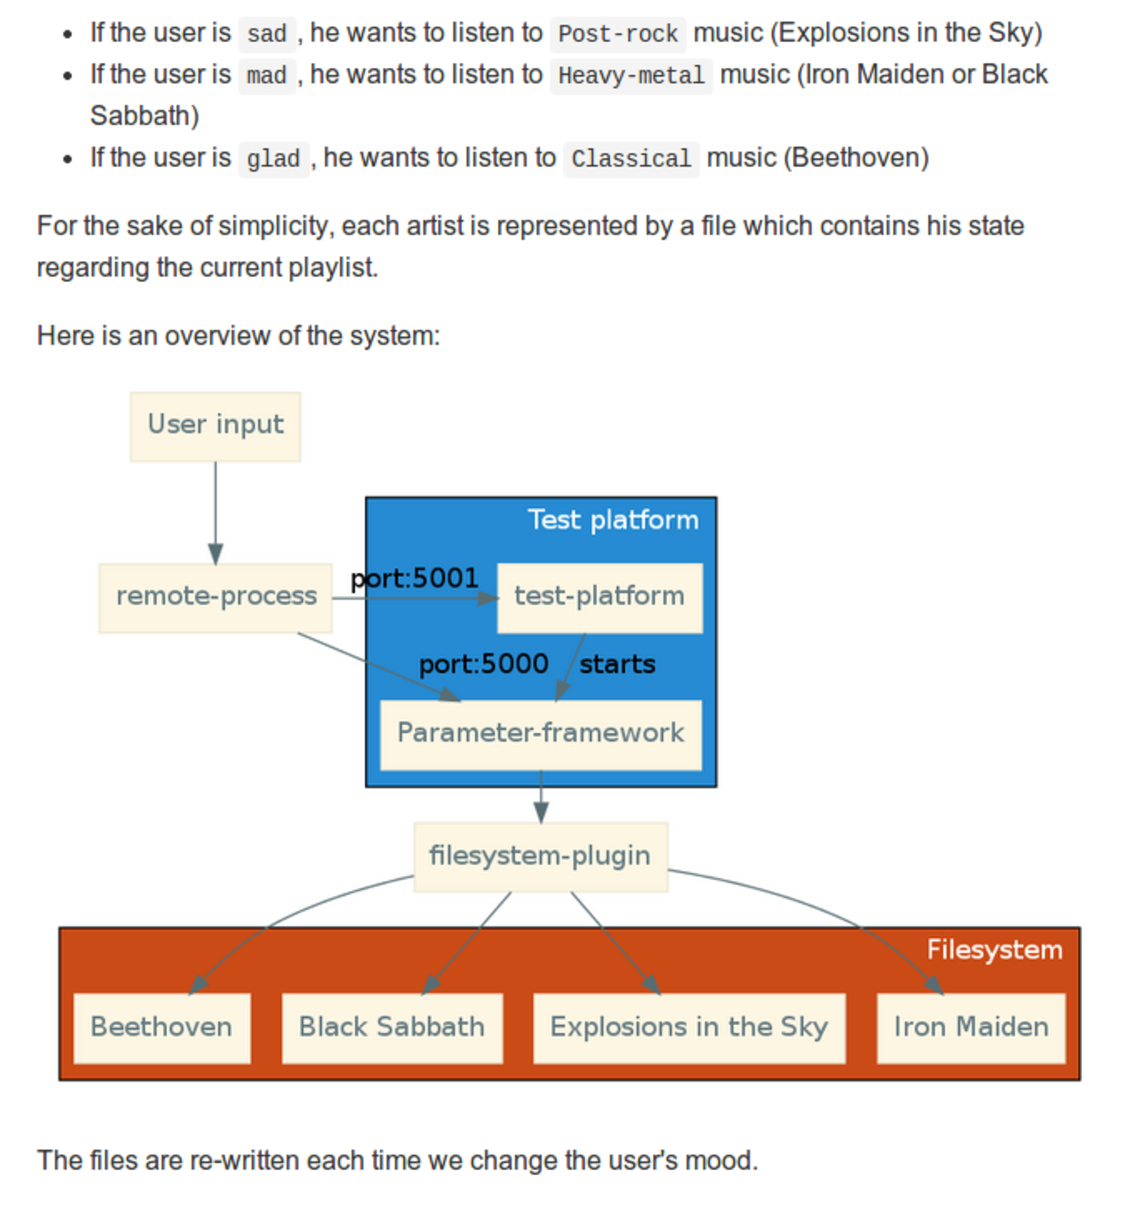
\includegraphics[height=0.5\textheight]{./src/img/tutos.pdf}
\end{figureGraphics}

At the moment, this documentation is used by other teams which need to train themselves on the \gls{pfw}.
There are more than \emph{450 lines} of text in these tutorials.
Some colleagues external to the team have been able to understand the concepts of the \gls{pfw} in 30 minutes
thanks to these tutorials.


% {{{2 ip plan
\subsection{Parameter-framework's intellectual property}
Before the code of the \gls{pfw} could be open-sourced, it had to be compliant with Intel's open-source policy.
Intellectual property is highly valuated at Intel. The \gls{pfw} needed to be released under
BSD license.
For that purpose, all the source files must contain the correct \emph{BSD license header}.
However, there are more than \emph{270 source files} which needed to be released on \gls{GitHub}.
Changing all those files by hand seems very time consuming, so I requested if a helper tool exists for that matter.

\subsubsection{license checker}
According to the team, there was no helper for changing software licenses easily.
Given the fact that I did not want to change 270 files by hand, I
wrote an internal tool in \gls{python} which performs the license check semi-automatically.
The script usage is quite straightforward and showed in listing \ref{code:license}.

\begin{code}[language=bash, caption=License checker usage, label=code:license]
usage: license_updater.py [-h] [--cpp | --mk] license root_location

Scans recursively trough directories to find source code which should be
updated with a new license header.

positional arguments:
    license        the license type: ['gpl', 'bsd', 'private']
    root_location  the directory to start scanning

optional arguments:
    -h, --help     show this help message and exit
    --cpp          (default) scan for C++ files: ('h', 'c', 'hpp', 'cpp')
    --mk           scan for Android make files: .mk
\end{code}

With this tool, it took less than half day of work to change the 270 involved files.


% {{{2 Align
\subsection{Code alignment}
One of the major problematics of open-sourcing a component is the way to version its source code.
The \gls{pfw} can receive contributions from several places:
\begin{description}
    \item[External contributions] can be done via \gls{GitHub}. The contributor forks the project, makes his development in a feature
        branch and then submits a pull request to the maintainer team which are members of the \emph{01org} organization.
    \item[Internal patches] are still done by Intel employees which need to add new features to the \gls{pfw}.
\end{description}
The difficulty is to maintain two \gls{git} repositories with the same code base. When receiving contributions on one code base, they
have to be ported to the other one. This should be done \emph{as soon as possible}. If that is not the case it would imply maintaining two different
code bases which is very expensive.

\subsection{Branch sync process}\label{sec:syncProcess}
Since we work internally on the \gls{pfw} and can receive external contributions via \gls{pullrequests},
it is quite difficult to keep both repositories in sync.
On figure \ref{fig:branch-process} we can see how we plan to synchronize the different code.

\begin{figureGraphics}{Final branch process}{fig:branch-process}
    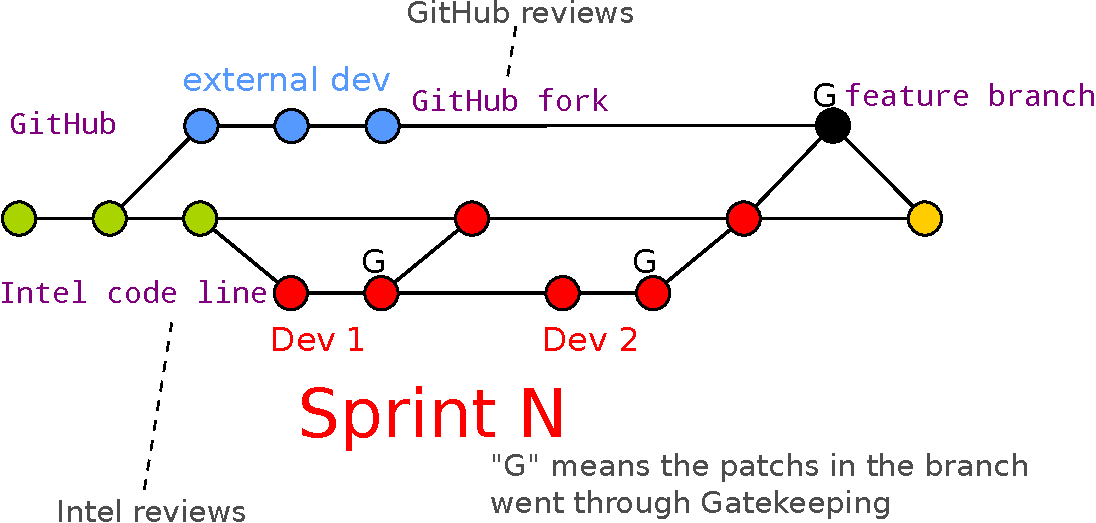
\includegraphics[width=\textwidth]{./src/img/branches-process-crop.pdf}
\end{figureGraphics}
At the end of every sprint, we are re-aligning the internal source tree with the one in \gls{GitHub}.
External contributions go trough a special feature branch, which is tested with the gatekeeping mechanism described in section \ref{sec:gatekeeping}.
If every test passes, the code is merged into Intel's codebase.

I worked on three different projects to set up this branch process:
\begin{itemize}
    \item The core component of the \gls{pfw}.
    \item The \gls{alsa} plugin.
    \item The filesystem plugin.
\end{itemize}

This was a very good exercise to improve my \gls{git} skill.

% {{{2 core align
\subsection{Core alignment}
The \gls{pfw} core is quite a big project, with about 30 000 lines of code.
Align the internal tree and the \gls{GitHub} version of this project required quite some work.
Some extra requirements apply on open-source projects, such as being compilable in a \gls{vanilla} \gls{aosp} environment.

There is a \gls{GitHub} organization which groups all Intel open-source projects. This
organization is called \emph{01org}. I joined it during my internship in order to have admin rights
on the projects I had to open-source.

The \gls{pfw} core is available on \gls{GitHub}\footnote{\url{https://github.com/01org/parameter-framework}}

% {{{2 fs plugin
\subsection{Filesystem plugin alignment}

The file system plugin is used for global access to the filesystem. This can be to
use \emph{/proc} entries for instance. I used this plugin as example in the rookie
documentation I wrote as described in section \ref{sec:tutorials}.

I also worked on an other example: \emph{controlling LEDs} via the filesystem
plugin on a Raspberry Pi.  This example was easy enough to be integrated into
the online documentation of the filesystem plugin, on \gls{GitHub}.

The filesystem plugin is available on \gls{GitHub}\footnote{\url{https://github.com/01org/parameter-framework-plugins-filesystem/}}

% {{{2 alsa plugin
\subsection{Alsa plugin alignment}

The \gls{alsa} plugin is used to handle \gls{alsa} (for desktop mostly) or TinyAlsa (for embedded \gls{android} devices mostly) subsystems.
For our internal uses, we patched some \gls{aosp} projects such as TinyAlsa which allows us to support proprietary controls.
The support of such controls was also implemented in the \gls{alsa} \gls{pfw} plugin. Since
we want to open-source the plugin, those proprietary features needed to be removed.

\subsubsection{Plugin refactoring}
The \gls{alsa} plugin used to be divided in two separate plugins: one for \gls{alsa} \emph{controls} and one for \gls{alsa} mixers.
This required the user to include them both if they need to use an \gls{alsa} subsystem since those plugins did not work as
standalone.

We decided to do a pair programming refactoring job to merge the two parts into one consistent plugin.
This allowed us to remove all the \emph{template} usage in the \gls{cpp} code.
The result is a far simpler and more elegant design which could be uploaded to \gls{GitHub}.

\subsubsection{Align on GitHub}
The \gls{alsa} \gls{pfw} plugin is used on within the Intel Audio \gls{hal}. It can also by used
on a linux desktop environement to handle \gls{alsa} mixers.

To demonstrate the power of this plugin, I wrote the README file which is on the
front page on this \gls{GitHub} project.  The README contains :
\begin{itemize}
    \item Build and install instructions
    \item Prerequisites for using this plugin
    \item A tutorial which details how to write the \gls{xml} files for this
    plugin in order to be able to change the master volume on a linux desktop.
\end{itemize}
I also reorganised some code within this plugin since we used to rely on proprietary \gls{aosp} modifications.
This plugin is now \gls{vanilla} \gls{aosp} compatible, and can be used if the \gls{pfw} is installed.

The \gls{alsa} plugin is available on \gls{GitHub}\footnote{\url{https://github.com/01org/parameter-framework-plugins-alsa/}}
 % WHAT I CREATED at work
\chapter{What I have learned}

\section{Android system development}

\section{Tools}
 % WHAT I have learned
\chapter{Conclusion}
\section{subsect}
\subsection{subsub}
Hello, world.
Lorem ipsum dolar

AAAA bscdde

\subsection{}

\section{Global conclusion}

%\bibliography{./src/biblio}
%\chapter{Annexes}

\section{Table des annexes}
\begin{description}
  \item[Opérations implémentées] Figure \ref{fig:opImpl} sur la page \pageref{fig:opImpl}
  \item[constants.vhd] Listing \ref{src:constants} sur la page \pageref{src:constants} 
  \item[cpu\_package.2.vhd] \ref{src:cpupackage} sur la page \pageref{src:cpupackage} 
  \item[memory.1.vhd] \ref{src:memory} sur la page \pageref{src:memory}
  \item[pipelineRegisters.vhd] \ref{src:pipelineReg} sur la page \pageref{src:pipelineReg}
  \item[registres.1.vhd] \ref{src:regs} sur la page \pageref{src:regs}
  \item[risc.0.vhd] \ref{src:risc} sur la page \pageref{src:risc}
\end{description}

\section{Liste des instructions implémentées}
      \begin{figureGraphics}{Liste des instructions implémentées}{fig:opImpl}
        \centering
        \begin{tabular}{|l|l|r|}
          \hline
          Catégorie  &  Instruction &  Implémenté \\
          \hline
          \hline
          Arithmétique  &  add  &  oui\\
          \hline
                         &  sub  &  oui\\
          \hline
                         &  addi  &  oui\\
          \hline
                         &  addu  &  oui\\
          \hline
                         &  subu  &  oui\\
          \hline
                         &  addiu  &  oui\\
          \hline
                Logique  &  and  &  oui\\
          \hline
                         &  or  &  oui\\
          \hline
                         &  xor  &  oui\\
          \hline
                         &  nor  &  oui\\
          \hline
                         &  andi  &  oui\\
          \hline
                         &  ori  &  oui \\ 
          \hline
                         &  xori  &  oui\\
          \hline
                         &  lsl  &  oui\\
          \hline
                         &  lsr  &  oui\\
          \hline
          \hline
             Chart. imm  &  lui  &  oui\\
          \hline
              Transfert  &  lb  &  oui\\
          \hline
                     de  &  lh  &  oui\\
          \hline
               données  &  lw  &  oui\\
          \hline
                         &  lbu  &  oui\\
          \hline
                         &  lhu  &  oui\\
          \hline
                         &  sb  &  oui\\
          \hline
                         &  sh  &  oui\\
          \hline
                         &  sw  &  oui\\
          \hline
          \hline
            Branchement  &  beq  &  oui\\
          \hline
           conditionnel  &  bne  &  oui\\
          \hline
                         &  bltz  &  oui\\
          \hline
                         &  blez  &  oui\\
          \hline
                         &  bgtz  &  oui\\
          \hline
                         &  bgez  &  oui\\
          \hline
                         &  bltzal  &  non\\
          \hline
                         &  bgezal  &  non\\
          \hline
                         &  slt  &  non\\
          \hline
                         &  sltu  &  non\\
          \hline
                         &  sltu  &  non\\
          \hline
                         &  sltiu  &  non\\
          \hline
          \hline
                   Saut  &  j  &  oui\\
          \hline
         Inconditionnel  &  jr  &  oui\\
          \hline
                         &  jal  &  oui\\
          \hline
                         &  jalr  &  oui\\
          \hline
        \end{tabular}
      \end{figureGraphics}

\section{Sources VHDL}

%change geom for source listing
\newgeometry{left=2.5cm,right=2.5cm}

\lstinputlisting[language=VHDL, caption=constants.vhd, label=src:constants]{../src/constants.vhd}
\lstinputlisting[language=VHDL, caption=cpu\_package.2.vhd, label=src:cpupackage]{../src/cpu_package.2.vhd}
\lstinputlisting[language=VHDL, caption=memory.1.vhd, label=src:memory]{../src/memory.1.vhd}
\lstinputlisting[language=VHDL, caption=pipelineRegisters.vhd, label=src:pipelineReg]{../src/pipelineRegisters.vhd}
\lstinputlisting[language=VHDL, caption=registres.1.vhd, label=src:regs]{../src/registres.1.vhd}
\lstinputlisting[language=VHDL, caption=risc.0.vhd, label=src:risc]{../src/risc.0.vhd}

\end{document}
